 \begin{figure*}[thb!]
 	\caption{Approach overview}
 	\centering
 	\label{fig:approach_overview}
 	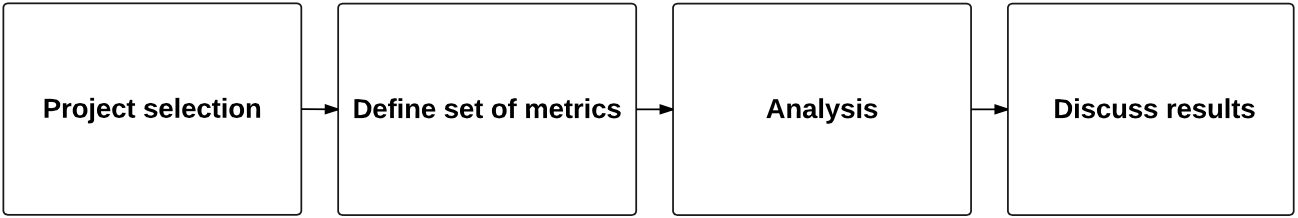
\includegraphics[width=1\textwidth]{figures/approach_overview}
 \end{figure*}

We ran our empirical study on 10 open source applications, 5 of then are written in JavaScript and the other 5 were written in Java. We present the approach overview for our study as shown in Fig.\ref{fig:approach_overview}. In this section we explain in detail how we realized the project selection, then we discuss metrics and particularities of the JavaScript language taken in consideration for this study and after that, we explain how we ran our analysis and finally we use the results to answer our research questions in section \ref{sec:rq}.

\subsection{Project Selection}


\begin{table*}\label{eval_table}\centering
	\caption{Proposed experiment projects with preliminary results of most recent version of release in our dataset}
	\begin{threeparttable}
		\scalebox{0.7}{
			\begin{tabular}{ccccccc}
				\toprule
				Name & Description &  {\# of JS files in latest release} & Number of Directories & LOC \footnote{Lines of code}& Number of Functions & Number of Statements  \\
				\addlinespace
				\midrule
				NPM & Package manager for JavaScript & 165 & 32 & 9,075 & 1,217 & 5,329  \\
				\addlinespace
				\midrule
				Node MySQL & A pure node.js JavaScript Client implementing the MySql protocol.  & 140 & 11& 4,720 & 667 & 3,317 \\			
				\addlinespace 	
				\midrule
				Esprima & A high performance, standard-compliant JavaScript parser written in JavaScript  & 34 & 6 & 83,385 & 4,862 & 29,002  \\
				\addlinespace		
				\midrule
				Grunt & The JavaScript Task Runner & 31 & 9 & 2,361 & 251 & 1,245 \\
				\addlinespace
				\midrule
				Node Redis & Redis client for node & 18 & 6 & 2,529 &  457 & 2,537   \\	
				\addlinespace 
				
			\end{tabular}
		}
	\end{threeparttable}
\end{table*}

\begin{table*}\label{tab:eval_java}\centering
	\caption{Proposed experiment projects with preliminary results of most recent version of release in our dataset}
	\begin{threeparttable}
		\scalebox{0.7}{
			\begin{tabular}{ccccccccc}
				\toprule
				Name & Description & {\# of java files in latest release} & Number of Directories & LOC & Number of Functions & classes & Number of Statements \\
				\addlinespace
				\midrule
				ElasticSearch & Open Source, Distributed, RESTful Search Engine 
				& 4,050 & 831 & 424,007 & 35,762 & 5,967 & 198,944 \\
				\addlinespace
				\midrule
				Gauva & Google Core Libraries for Java 6+ & 799 & 28 & 90,401 & 11,769 & 1,644 & 32,698\\    
				\addlinespace 
				\midrule
				JodaTime & Joda-Time is the widely used replacement for the Java date and time classes. & 327 & 15 & 84,855 & 9,560 & 473 & 50,609 \\
				\addlinespace    
				\midrule
				Jsoup & Jason library for java & 80 & 14 & 13,672 & 1,487 & 154 & 7,980 \\
				\addlinespace
				\midrule
				JUnit & Unit test framework for java & 392 & 73 & 26,079 & 3,479 & 1,063 & 7,972  \\   	
				\addlinespace 
			\end{tabular}
		}
	\end{threeparttable}
\end{table*}

\subsection{Define set of metrics}

Lehman suggests using the number of “modules” as the best way to measure the size of a large software system \cite{Lehman1997METRICS}. However, we decided to use the number of uncommented lines of code (“uncommented LOC”) like the way Godfrey et al \cite{Godfrey2000ICMS} did the evolution study on Linux Kernel. On the other hand we measure the comment lines and the ratio of comments to lines of codes, and based on that we can infer how much developers tend to put comments within their codes. We have to consider hidden corners that can mislead results, for example descriptive comments are totally different to the lines of codes that got commented because of refactoring or changes which consider as light-weight code smells within the code.

We want to measure various aspects of the growth of these applications by having metrics such as number of files, lines of code, number of functions and statements. We also measure amount of duplications known as clones in terms of lines of codes, blocks and files. We measure the cyclomatic complexity over time which the metric is calculated as following. Whenever the control flow of a function splits, the complexity counter gets incremented by one. Each function has a minimum complexity of 1. The control flow can split by conditional statements like if/else, switch case and so on. This metric is also known as also known as McCabe metric
We use the term “source file” to mean any file whose name ends with “.js” and also we removed folders containing external libraries which is usually located at \textit{lib} or \textit{node\_modules}. 

We also measure the amount of object oriented principles that JavaScript developers use in their day to day software development. We think if we quantify the amount of reusable parts (i.e classes) in these projects, there are some valuable reasons laid down related to evolution behind these techniques. Consequently we use a project, known as JSDeodorant to find class declarations and places developers instantiate objects.
In the rest of this section we describe how developers create objects in JavaScript and how they mimic object oriented class definitions without having direct language support in the specification of language.

\noindent\textbf{Creation Types:} Following we explain different types of object creation no matter if they are built-in type or user-defined. 
%\subsubsection{Creation Types}

\medskip
\noindent\subsubsection{Array Literal Expression}
%\duptype{\textbf{Type I}: \textit{Array Literal Expression}.}

it creates a string array consisting of three creations possible in JavaScript elements and is assigned to variable “cars” using a binary operator (with two operand and equal operator). 
\medskip
\begin{lstlisting}[caption={Array literal expression},label={lst:array_literal},language=JavaScript]
var cars = ['Saab', 'Volvo', 'BMW'];
\end{lstlisting}
A JavaScript array is initialized with the given elements, except in the case where a single argument is passed to the Array constructor and that argument is a number. Note that this special case only applies to JavaScript arrays created with the Array constructor, not array literals created with the bracket syntax.
\\
%\break
%\duptype{\textbf{Type II}: \textit{Array Creation using \textbf{new} keyword}.}
\noindent\subsubsection{Array Creation using \textbf{new} keyword}

The Array constructor function with using the “New” keyword creates an array of three elements and then assigned the created object to variable “planes” using binary operator. Using the more verbose method: \textit{new Array()} instead of array literal expression does have one extra option in the parameters: if you pass a number to the constructor, you will get an array of that length. 

\medskip
\begin{lstlisting}[caption={Array constructor},label={lst:array_constructor},language=JavaScript]
var planes= new Array('Boeing', 'Airbus', 'Bombar- dier');
\end{lstlisting}

\noindent\subsubsection{Object Literal Expression}

%\duptype{\textbf{Type III}: \textit{Object Literal Expression}.}

The created object is basically singletons with variables/methods that are all public. An object literal is a comma-separated list of name-value pairs wrapped in curly braces. Object literals encapsulate data, enclosing it in a tidy package. This minimizes the use of global variables which can cause problems when combining code. If any of the syntax rules are broken, such as a missing comma or colon or curly brace, a JavaScript error will be triggered. No need to invoke constructors directly or maintain the correct order of arguments passed to functions.
\begin{lstlisting}[caption={Object literal expression},label={lst:object_literal_expression},language=JavaScript] 
var myObj = {
	myMethod: function(params) {
		// ...do something
	}
};
\end{lstlisting}

\noindent\subsubsection{Function Constructor}
%\duptype{\textbf{Type IV}: \textit{Function Constructor}.}

Listing \ref{lst:function_constructor}, shows the function constructor, there we define a function that should start with an uppercase letter by convention (to inform call sites use this function with “new” keyword). The Function constructor creates a new Function object and in JavaScript every function is actually a Function object.

Parameters are Names to be used by the function as formal parameter names. Each must be a string that corresponds to a valid JavaScript identifier or a list of such strings separated with a comma. Functions created with the Function constructor do not create closures to their creation contexts; they always are created in the global scope.

When running them, they will only be able to access their own local variables and global ones, not the ones from the scope in which the Function constructor was called.

\begin{lstlisting}[caption={Function constructor},label={lst:function_constructor},language=JavaScript] 
function Employee(name){
	this.name = name;
	this.getName = function(){
		return this.name;
	};	
};
var emp = new Employee ('John');
\end{lstlisting}